\pagestyle{plain} \pagenumbering{arabic}

\begin{center}
{\Large{\bf \mytitle}}
\end{center}
\vspace{-0.1in}

\Section{Introduction}
\label{sec:intro}


The past decade has produced stunning advances in computer vision. Real-time face detection that was introduced at the turn of the millennium is now commonplace in personal electronic devices. Face recognition has evolved from being just a research topic to a widely-used tool for managing personal and community photo collections. Built on academic research from the 1990's, we now have systems like Microsoft Photosynth and Google Earth that can automatically reconstruct three-dimensional models from large, unstructured photo collections. And thanks to the growing availability of annotated image collections and research in vision and machine learning, our ability to distinguish between object categories has improved dramatically, enabling applications from image search to product identification.

If the purpose of computer vision is to extract from image data useful information about the world, it is clear that we now have useful, functioning vision systems for certain types of information. Yet, there are aspects of the world to which computer vision systems, relative to their human counterparts, remain quite blind. Prominent among these are the \emph{social interactions} and \emph{social relationships} between people. This is information is critical for humans as they navigate the world, making decisions about which table to join at a banquet; which schoolmates to invite to a dinner party; which colleagues to approach to enact change; or whether or not to intervene in a questionable interaction between strangers.


We propose to develop foundations for computer vision systems that are socially aware. These systems will extract, from images and videos of human gatherings, useful information about the types of social interactions that occur within these gatherings. And by enumerating the different types of interactions that occur over time in large image and video collections, they will extract useful information about the underlying \emph{social network}---the set of social relationships that exist among the observed individuals, groups, and communities. In other words, we seek to use computer vision systems as a new `sensor' from which we recover the underlying social network (Fig. \ref{fig:intro}).

Why is vision an important source of social network information? Social network information can come from various sources, but vision is an important one. Facial expressions, gestures, and body poses are critical signals for understanding the interactions and relationships between people, and the only way to get these are from images and videos. Also, it is not just important to understand the type of interaction, but also the context of the scene in which it occurs.

Our project has three main parts:

1. Detecting and recognition of interaction categories. Relatively mature in images due to face detection, person detection, and pose estimation. But largely unsolved in videos. We will address the questions including 1) How do we represent an interaction category? 2) How do we identify in a long video of a large gathering 3) when this interaction occurs, and 4) who it involves? To do so, we will develop approaches to learn effective and efficient interaction detector for  a given set of categories. These socially-salient interaction categories may arise from sociology \cite{Kendon1990,Ekman,Hoyle,Tannen,Goodwin2000,Goldin,Goodwin2007,Kendon2010,Lazer2009}, but this does not scale in novel environments and applications. Therefore, we will develop approaches to learn representations for new categories from image/video collections in a semi-supervised or unsupervised manner.

2. Inferring social network information from detected interactions. We will design mechanisms by which we distill ties or affinities between social members from multiple heterogeneous visual cues, and in particular accounting for the multi-view effect in a practical social network. To achieve robustness, our research will especially focus on noise-resilient methods for mapping image targets to the identities of the members, as well as novel algorithms to the case of incomplete and noisy outputs from the social network estimator due to various types of imperfection incurred from missed detections; mis-classified interactions, and a large fraction of missing observations.

3. Data collections and challenge problems. We will collect datasets to evaluate our methods and design challenge problems to engage our colleagues in this research agenda. To do this, we will address the challenges of enabling reproducible research while preserving privacy.

\begin{figure}[t!]
\begin{center}
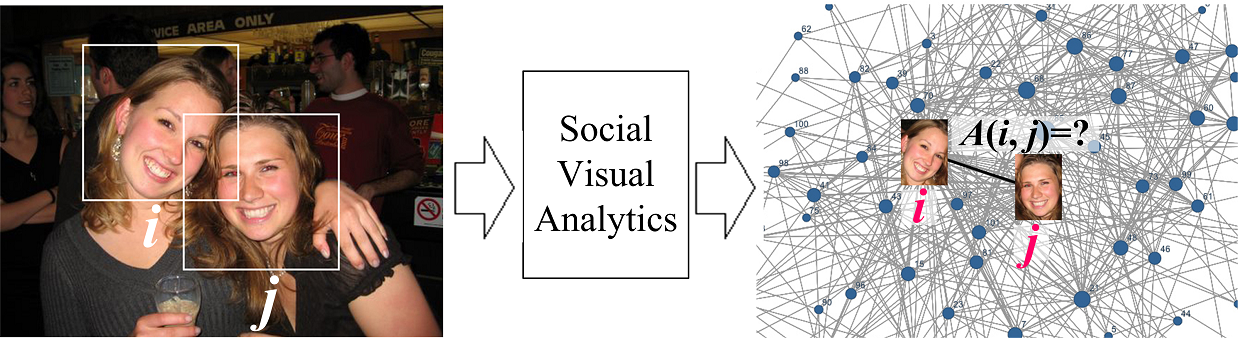
\includegraphics[width=\columnwidth]{intro}
\end{center}
\vspace{-0.25in} \caption{\captionsize 
Social visual analytics: A computer vision approach to `sense' a social network. \label{fig:intro}\afterfigspace}
\end{figure}

This lays the foundation for socially-aware computer vision systems. These systems will transform security, anti-terrorism, autonomous visual analytics, augmented reality, human computer interaction, human resource planning, operations research, game theory and e-commerce, and identify recognition. 

This research will be carried out by a team with established expertise in recognition of identities, activities, and interactions, as well as collecting and analyzing social image and video collections. PI Todd Zickler has pioneered research on the use of social network context to improve identity recognition~\cite{Stone2008,Stone2010} and led the implementation of a camera-based system for long-term observation of social interactions in an interactive classrooms (Section~\ref{sec:sys}). PI Ruonan Li has substantial expertise in group interactions recognition~\cite{LiIJCV2012}, analyzing human activities and behaviors~\cite{Li2010,LiPAMI2012}, and domain adaptation methods for learning appearance models when annotated training data is difficult or expensive to acquire~\cite{LiZickler2012,Li2011}. 

The proposal is organized as follows. Following a discussion of related work in Section 2, we being our proposed research in Section 3.1 by discussing representations for social interactions and the problem of detecting an interaction in a long video of a large social gathering. In particular, we discuss how this technology will help us to discover and learn salient interaction categories in semi-supervised and unsupervised scenarios. Section 3.2 moves on to describe how to infer social network information from interactions that are detected over time and space in large image and video collections, with a focus on robustly associating identities to targets in the images/videos and effectively reconstructing noisy and incomplete multi-view netowrks. Finally, Section 3.3 describes data collection and challenge problems for evaluation.



